\documentclass[a4paper,11pt]{article}

\usepackage{mlsubmit}
\usepackage{tikz}
\tikzset{
  treenode/.style = {shape=rectangle, rounded corners,
                     draw, align=center,
                     top color=white, bottom color=blue!20},
  root/.style     = {treenode, font=\Large, bottom color=blue!20},
  env/.style      = {treenode, font=\ttfamily\normalsize},
  dummy/.style    = {circle,draw}
}

\begin{document}

\initmlsubmision{2}{Talla Aravind Reddy}{14746}														

\begin{mlsolution}

\section{Name:}
No. 
\\Because whether a professor is a good advisor or not does not depend on their name. 
\\Therefore, although there might be a correlation between some function of the name(for example whether the first letter is after `g' or before `g' in the alphabet) and the good/not good advising, it is only limited to the data set we have and it would not be true if we had a very large dataset. 
\\Therefore, we should ignore this attribute while building our decision tree.

\section{Perfect classification of given dataset:}
No.
\\Look at the 4th and 6th entries of the given dataset. 
\\Both of them have the same values for all the important attributes(i.e all except name) yet they have different values for whether the advisor is Good/Not Good. 
\\Therefore, any classification algorithm we come up with can only be correct for either entry 4 or entry 6 but not both simultaneously(if it is a deterministic algorithm).
\\In this case, randomised algorithms might give correct results for both entries in some runs of the algorithm. But they are not perfect since they give wrong results also in other runs.

\section{Decision Tree:}
\begin{center}
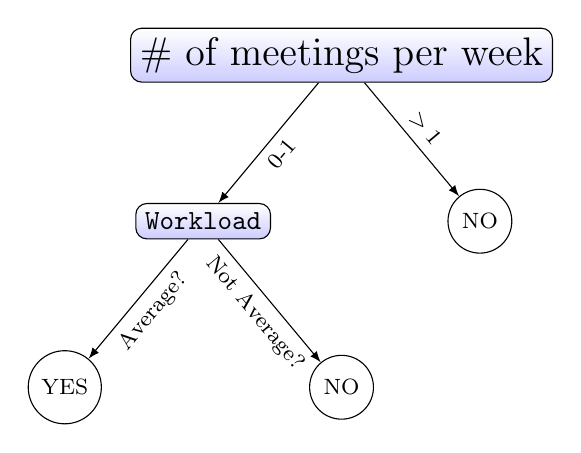
\begin{tikzpicture}
  [
    grow                    = down,
    sibling distance        = 10em,
    level distance          = 6em,
    edge from parent/.style = {draw, -latex},
    every node/.style       = {font=\footnotesize},
    sloped
  ]
  \node [root] {\# of meetings per week}
  child { node [env] {Workload}
    	child { node [dummy] {YES}
        edge from parent node [below] {Average?} }
      child { node [dummy] {NO}
              edge from parent node [above, align=center]
                {}
              node [below] {Not Average?}}
             edge from parent node [below] {0-1} }
    child { node [dummy] {NO}
              edge from parent node [above] {$> 1$} };
\end{tikzpicture}
\end{center}


\subsection{Information gain values:}
At root node, information gains for 
\\$Size = 0.067, Like = 0.031, Workload = 0.061, Meetings = 0.251 \implies Meetings$
\\For depth one node, where \# meetings = 0-1, information gains for 
\\$Size = 0.114, Like = 0.035, Workload = 0.439 \implies Workload$

\subsection{Further splitting:}
For root node's children, \# meetings $> 1$ is not split into $2-3$ and $>3$ because all the entries which fall into these categories are classified in the `No' class.
\\For  Workload's children, the `Average' child has all values as YES(for average workload 3/3) and the `Not average' child has majority NO values(6 out of 8).

\iffalse
\begin{table}[h!]
\centering
{\small
\begin{tabular}{| c | l | c | c | c | c | c |}
	\hline
	S.No. & Name  & $\substack{\text{Size of}\\\text{research group}}$ & $\substack{\text{Like the}\\\text{research area?}}$ & $\substack{\text{Average}\\\text{workload?}}$ & $\substack{\text{\# of meetings}\\\text{per week}}$ & $\substack{\text{Good}\\\text{advisor}}$? \\ \hline
	4 & Prof. C. Binns & medium & no  & heavy & $0-1$ & no \\ \hline
	5 & Prof. A. Sinistra & large  & no  & heavy & $0-1$ & no \\ \hline
	6 & Prof. S. Snape & medium & no  & heavy & $0-1$ & yes \\ \hline
	10 & Prof. R. Hooch & medium & no  & light & $0-1$ & no \\ \hline
	12 & Prof. A. P. W. B. Dumbledore & medium & yes & light & $0-1$ & yes \\ \hline
	14 & Prof. H. Slughorn & medium & no  & heavy & $0-1$ & no \\ \hline
	15 & Prof. Q. Quirrell & large  & yes & heavy & $0-1$ & no \\ \hline
\end{tabular}
}
\end{table}
\fi

\end{mlsolution}

\begin{mlsolution}
This is for Question 2

\end{mlsolution}

\begin{mlsolution}


Lorem ipsum dolor sit amet, consectetur adipiscing elit. Duis feugiat vehicula dolor, sed ultricies leo. Phasellus euismod dictum felis in euismod. Proin pretium vel neque in placerat. Proin imperdiet egestas vulputate. Etiam faucibus accumsan ante non viverra. Duis ultrices ac odio vel sodales. In maximus gravida dolor, ut commodo lacus. Pellentesque ante massa, venenatis id aliquam et, posuere sed dui. Duis dignissim justo sit amet augue posuere fringilla. Suspendisse at nisi gravida, mattis justo sit amet, elementum elit. Praesent et massa ornare, consequat dui eget, ornare risus. Duis est nibh, sollicitudin nec mattis non, mattis in leo. Donec finibus justo sed massa sagittis, non fermentum nibh dictum. Pellentesque et congue purus. Donec porta pretium porttitor.

Morbi euismod risus eu tortor ornare malesuada. Nunc sed sollicitudin neque, efficitur rhoncus tellus. Cras malesuada augue arcu. Sed sem odio, tincidunt quis laoreet ac, facilisis ut nibh. Quisque gravida dolor at egestas aliquam. Aenean mollis massa sit amet enim mattis, vel fermentum tortor facilisis. Donec pellentesque est velit, vitae posuere lorem tristique ut.

\begin{figure}[th]%
\centering
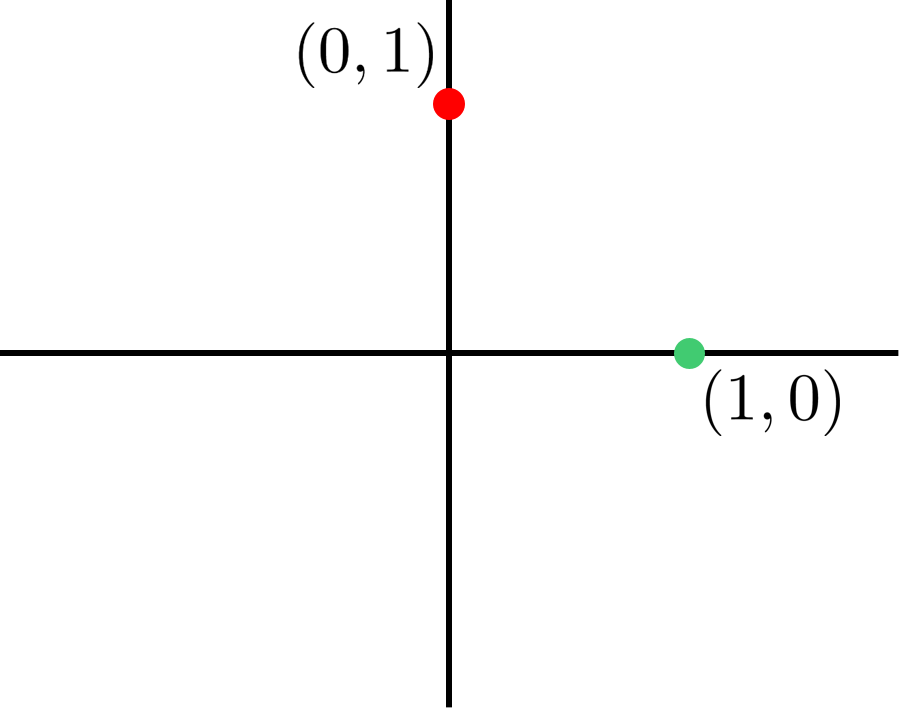
\includegraphics[width=0.4\columnwidth]{proto_blank.png}%
\hfill
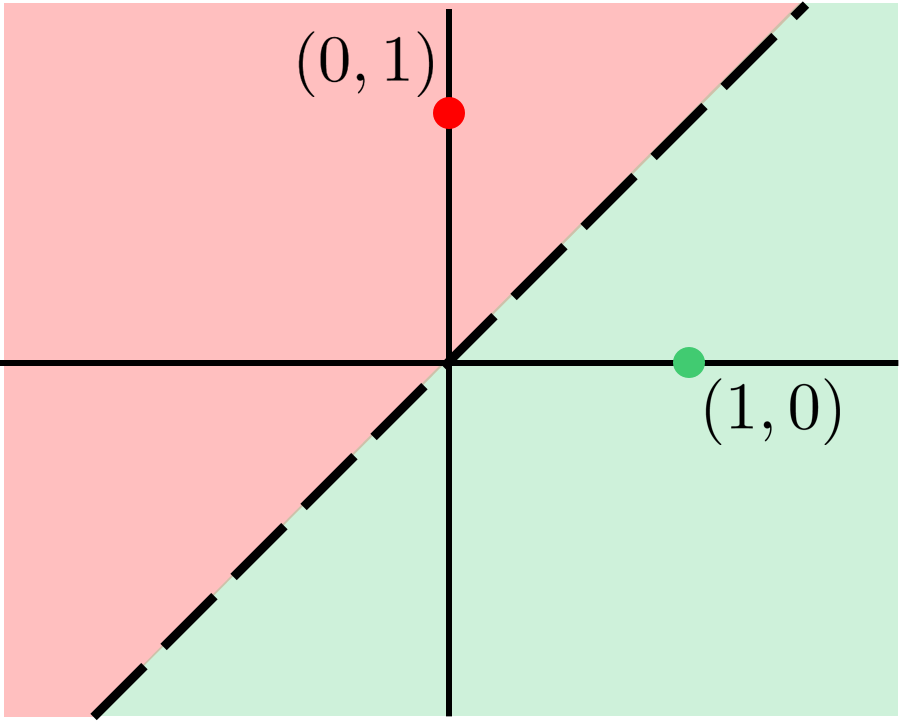
\includegraphics[width=0.4\columnwidth]{proto_euclid_sample.png}%
\caption{Learning with Prototypes: the figure on the left shows the two prototypes. The figure on the right shows what the decision boundary if the distance measure used is $d(\vz^1,\vz^2) = \norm{\vz^1-\vz^2}_2$, for any two points $\vz^1,\vz^2 \in \bR^2$. The decision boundary in this case is the line $y = x$.}%
\label{fig:proto}%
\end{figure}

Fusce pulvinar convallis lobortis. Mauris iaculis lacus vitae dui suscipit, ut ornare neque placerat. In mattis malesuada rutrum. Vivamus consectetur tempus ex sit amet aliquam. In blandit libero at mi rutrum, nec iaculis orci cursus. Maecenas a dolor lorem. Donec pretium turpis sapien, dapibus sollicitudin odio scelerisque eget. Maecenas egestas tellus a quam scelerisque, et pretium magna condimentum. In dapibus feugiat ornare. Nunc eget nulla convallis, laoreet tortor nec, convallis dui. Etiam in leo vitae nulla facilisis congue. Curabitur blandit sodales augue. Vivamus et aliquam orci, non suscipit elit. Quisque vestibulum lacus at velit congue semper.

Nulla efficitur risus nunc, in posuere turpis tempor eget. Sed efficitur id tellus non vestibulum. Praesent elementum condimentum sollicitudin. Integer eget quam dictum, varius est sit amet, aliquam mauris. Vestibulum ante ipsum primis in faucibus orci luctus et ultrices posuere cubilia Curae; Morbi in pretium dui. Sed luctus magna rutrum ex mollis, ut blandit lacus tincidunt. In tincidunt urna neque, placerat consequat velit sagittis id. Morbi pretium maximus fermentum. Interdum et malesuada fames ac ante ipsum primis in faucibus. Duis vehicula efficitur rhoncus. Nullam lacinia semper scelerisque. Maecenas eleifend nisi et ante auctor, a tincidunt arcu molestie. Aenean faucibus feugiat arcu ac mattis.

Morbi quis suscipit sapien. Pellentesque pulvinar fermentum tellus at malesuada. Nam id metus vitae risus dignissim laoreet. Pellentesque massa velit, vehicula in convallis et, vestibulum sed turpis. In venenatis massa vel mattis tincidunt. Donec varius faucibus elit, in blandit metus interdum sit amet. Nullam vel nibh non nisl mollis volutpat. Donec cursus iaculis lorem, id elementum metus iaculis nec. Cras a diam porttitor, suscipit dolor id, vestibulum nisi. Morbi maximus mauris a iaculis hendrerit. Duis rutrum quam in ex lobortis gravida. Aenean iaculis lacinia metus. Fusce sit amet dignissim elit, sed sodales lacus. Mauris ac neque finibus, bibendum tortor id, scelerisque neque. In nec quam ullamcorper, egestas sem ut, iaculis ante. Nam porta diam ut lacus sagittis euismod. 
\end{mlsolution}

\begin{mlsolution}
 Lorem ipsum dolor sit amet, consectetur adipiscing elit. Duis feugiat vehicula dolor, sed ultricies leo. Phasellus euismod dictum felis in euismod. Proin pretium vel neque in placerat. Proin imperdiet egestas vulputate. Etiam faucibus accumsan ante non viverra. Duis ultrices ac odio vel sodales. In maximus gravida dolor, ut commodo lacus. Pellentesque ante massa, venenatis id aliquam et, posuere sed dui. Duis dignissim justo sit amet augue posuere fringilla. Suspendisse at nisi gravida, mattis justo sit amet, elementum elit. Praesent et massa ornare, consequat dui eget, ornare risus. Duis est nibh, sollicitudin nec mattis non, mattis in leo. Donec finibus justo sed massa sagittis, non fermentum nibh dictum. Pellentesque et congue purus. Donec porta pretium porttitor.

Morbi euismod risus eu tortor ornare malesuada. Nunc sed sollicitudin neque, efficitur rhoncus tellus. Cras malesuada augue arcu. Sed sem odio, tincidunt quis laoreet ac, facilisis ut nibh. Quisque gravida dolor at egestas aliquam. Aenean mollis massa sit amet enim mattis, vel fermentum tortor facilisis. Donec pellentesque est velit, vitae posuere lorem tristique ut. 
\end{mlsolution}
					
\end{document}